\chapter{The concept of black hole 2: Non-expanding horizons}
\label{s:neh}

\minitoc

\section{Introduction}

Having discussed in depth the geometry of null hypersurfaces in Chap.~\ref{s:def}
we move forward here to distinguish a null hypersurface representing a black hole event horizon from, let us say, a future light cone. We do it for black holes
\emph{in equilibrium}. Indeed, for such black holes, it is quite natural
to assume a vanishing expansion. This leads us the concept of \emph{non-expanding
horizon} (Sec.~\ref{s:neh:neh}). A special kind of these objects is that
of \emph{Killing horizons} (Sec.~\ref{s:neh:Killing_hor}). Actually, we shall
see in Chap.~\ref{s:sta} that the event horizon of a black hole in equilibrium
must be a Killing horizon.


%%%%%%%%%%%%%%%%%%%%%%%%%%%%%%%%%%%%%%%%%%%%%%%%%%%%%%%%%%%%%%%%%%%%%%%%%%%%%%%%%%%%%%%%

\section{Non-expanding horizons} \label{s:neh:neh}

\subsection{Motivation and definition}

Having discussed in depth the geometry of null hypersurfaces, and in particular
their expansion, let us make an attempt to distinguish a black hole event
horizon from, let us say, a future light cone.
To get the localized behaviour mentioned in the black hole naive definition
of Sec.~\ref{s:def:first_defin}, we could demand that the area of the
spacelike cross-sections remains constant, in other words that
the expansion along the null normal vanishes. Hence the definition:\\
A \defin{non-expanding horizon}\index{non-expanding!horizon}\index{horizon!non-expanding --} is a null hypersurface $\Hor$ having the
topology (\ref{e:def:H_topology}):
\be
    \Hor \simeq \R \times \Sp,
\ee
where $\Sp$ is a closed manifold of dimension $n-2$,
and such that the expansion of $\Hor$ along any null normal $\wl$ vanishes
identically:
\be
    \theta_{(\wl)} = 0 .
\ee
Note that, given the scaling law (\ref{e:def:rescale_lambda}),
if $\theta_{(\wl)} = 0$ for some normal $\wl$, then  $\theta_{(\wl')} = 0$
for any other normal $\wl'$. Hence the definition of a non-expanding horizon
does not depend on the choice of the null normal.

As we shall discuss in detail in Chap.~\ref{s:sta}, this definition captures only
the event horizon of black holes in equilibrium.

\begin{example}[Schwarzschild horizon]
In view of Eq.~(\ref{e:def:theta_Schw_hor}), we may assert that the
Schwarz\-schild horizon considered in Examples~\ref{x:def:Schw_hor}, \ref{x:def:Schw_hor2},
\ref{x:def:Schw_hor3}, \ref{x:def:Schw_hor4}, \ref{x:def:Schw_hor5}, \ref{x:def:Schw_hor6},
\ref{x:def:Schw_hor7}, \ref{x:def:Schw_hor8} and \ref{x:def:Schw_hor9}
of Chap.~\ref{s:def}
is a non-expanding horizon.
\end{example}

\begin{hist}\label{h:neh:NEH}
The concept of non-expanding horizon has been introduced by P.~H\'a\'\j i\v{c}ek
in 1973 under the name of \emph{totally geodesic null hypersurface} \cite{Hajic73a}
or \emph{perfect horizon} \cite{Hajic73b,Hajic74}.
The terminology \emph{non-expanding horizon} is due to A.~Ashtekar, S.~Fairhurst
and B.~Krishnan in 2000 \cite{AshteFK00} (see also \cite{AshteBL02}).
\end{hist}

\subsection{Invariance of the area}

Given a cross-section $\Sp$ of $\Hor$, the area\index{area!of a cross-section} of $\Sp$, with respect to the spacetime metric $\w{g}$, is [cf. Eqs.~(\ref{e:def:A_wepsS_dx}) and (\ref{e:def:A_sqrt_q})]
\be \label{e:neh:total_area}
    A = \int_{\Sp} \wepsS(\D\w{x}_{(2)},\ldots,\D\w{x}_{(n-1)})
        = \int_{\Sp} \sqrt{q} \, \D x^2 \cdots \D x^{n-1} ,
\ee
where $x^a = (x^2, \ldots, x^{n-1})$ is a coordinate system on $\Sp$ and $q$ is
the determinant with respect to these coordinates of the Riemannian metric $\w{q}$
induced by $\w{g}$ on $\Sp$.

A direct consequence of the definition of a non-expanding horizon is that
$A$ does not depend on the choice of the cross-section $\Sp$.
\begin{proof}
Let $\Sp'$ be a second cross-section of $\Hor$ and let $\wl$ be a field of null normals
of $\Hor$. Along the null geodesic generators of $\Hor$, we can always choose a parameter $\lambda$ associated with $\wl$ (i.e. such that $\wl = \D/\D\lambda$ along a given null geodesic generator)
such that $\lambda=0$ on $\Sp$. By the very definition of a cross-section,
any null geodesic generator $\Li$ of $\Hor$ intersects $\Sp'$ at a single point. Let
$\lambda_0$ be the value of $\lambda$ at this point. We may then introduce
a new parameter along $\Li$ as follows:
\[
      \lambda' = \frac{\lambda}{\lambda_0} .
\]
If we repeat this for all null geodesic generators of $\Hor$, we obtain a parametrization
of all the null geodesic generators that satisfies $\lambda'=0$ on $\Sp$ and $\lambda'=1$
on $\Sp'$. Let $\wl'=\D/\D\lambda'$ be the (null) tangent vector associated
with $\lambda'$. We may then say that the cross-section $\Sp'$ is deduced
from $\Sp$ by the Lie dragging of $\Sp$ along $\wl'$ by a parameter $\delta\lambda'=1$.
More precisely, we may considered that $\Sp'$ is deduced from $\Sp$ by a
continuous deformation, represented by a 1-parameter family $(\Sp_{\lambda'})$
of cross-sections such that $\Sp_0 = \Sp$ and $\Sp_1 = \Sp'$. Associated
with this family is a real-valued function $\lambda' \mapsto A(\lambda')$
given the area of each element $\Sp_{\lambda'}$. By the very definition
of the expansion along $\wl'$ [Eq.~(\ref{e:def:def_expansion})], we have then
\[
    \frac{\D A}{\D\lambda'} = \int_{\Sp_{\lambda'}} \theta_{(\wl')} \, \delta A .
\]
If $\Hor$ is a non-expanding horizon, then $\theta_{(\wl')}=0$ and it follows
that $A(\lambda')$ is a constant function. Hence the area of $\Sp'$ is equal
to that of $\Sp$.
\end{proof}
Given that the quantity $A$ defined by (\ref{e:neh:total_area})
takes a unique value whatever the cross-section $\Sp$,
we call it the \defin{area of the non-expanding horizon}\index{area!of a non-expanding horizon}
$\Hor$.

\begin{example}[Schwarzschild horizon]
The area of the Schwarzschild horizon is readily computed from
the metric (\ref{e:def:q_S_Schw_hor}):
$q_{ab} \D x^a \D x^b = 4m^2 \left( \D\th^2 + \sin^2\th \D^2\ph \right)$;
we get
\[
     A = 16\pi m^2 .
\]
\end{example}

\subsection{Trapped surfaces}

If there is a natural concept of \emph{outer}/\emph{inner} for $\Hor$, for
instance the outer region being the one that contains an asymptotically flat end,
and if the transverse null normals $\w{k}$ point to the inner region, then
the property $\theta_{(\wl)}=0$ means that any cross-section $\Sp$ of the
non-expanding horizon $\Hor$ is a
\defin{marginally outer trapped surface}\index{marginally!outer trapped surface}\index{trapped!surface!marginally outer --}
(often abridged as \defin{MOTS}\index{MOTS}). This definition is due to
Hawking \cite{Hawki73}, an
\defin{outer trapped surface}\index{outer!trapped surface}\index{trapped!surface!outer --}
would be one for which $\theta_{(\wl)}\leq 0$.

\begin{figure}
\vspace{5cm}
%\centerline{\includegraphics[width=0.6\textwidth]{}}
\caption[]{\label{f:neh:expansions_flat} \footnotesize
Inward and outward expansions of a closed spacelike surface in Minkowski
spacetime.}
\end{figure}


This definition is related to, but distinct from, the definition of a
marginally trapped surface by Penrose \cite{Penro65}: a $(n-2)$-dimensional
submanifold $\Sp$ of $\M$ is a \defin{trapped surface}\index{trapped!surface}
 iff (i) $\Sp$ is
closed (i.e. compact without boundary), (ii) $\Sp$ is spacelike and (iii)
the two systems of null geodesics emerging orthogonally from $\Sp$ converge
locally at $\Sp$, i.e. they have negative expansions:
\be
    \theta_{(\wl)} < 0 \quad\mbox{and}\quad \theta_{(\w{k})} < 0 ,
\ee
where the expansion along $\w{k}$ is defined in the same way as that along
$\wl$ [cf. Eq.~(\ref{e:def:theta_l_all})]:
\be
    \theta_{(\w{k})} := \lim_{\varepsilon\rightarrow 0} \frac{1}{\varepsilon}
    \frac{\delta A^{(\w{k})}_\varepsilon - \delta A}{\delta A}
        = \frac{1}{2} \Lie{\w{k}} \ln q
        = \frac{1}{2} \, q^{\mu\nu} \Liec{k} q_{\mu\nu}
        = q^{\mu\nu} \nabla_\mu k_\nu ,
\ee
$\delta A^{(\w{k})}_\varepsilon$ begin the area of the surface element
that is deduced from the surface element of area $\delta A$ on $\Sp$ by the
Lie dragging along $\w{k}$ by a parameter $\varepsilon$.
The limit case $\theta_{(\wl)} = 0$ and $\theta_{(\w{k})}<0$ correspond
to the so-called \defin{marginally trapped surface}\index{marginally!trapped!surface}.

In a flat spacetime (Minkowski), given any spacelike surface,
one has $\theta_{(\wl)} > 0$ and $\theta_{(\w{k})} < 0$ (cf. Fig.~\ref{f:neh:expansions_flat}), so there
is no trapped surface.

Cross-sections of a non-expanding horizon are usually marginally trapped surfaces
(cf. the example below).
However there exist some pathological situations for
which $\theta_{(\w{k})} > 0$ at some points of $\Sp$ \cite{GerocH82}.

\begin{example}
Let us consider a cross-section $\Sp$ of the Schwarzschild horizon as
defined in Example~\ref{x:def:Schw_hor4} of Chap.~\ref{s:def}.
Computing $q^{\mu\nu} \nabla_\mu k_\nu$ from the components $k_\nu$
given by (\ref{e:def:l_k_forms_Schw_hor}) we get (cf. Appendix~\ref{s:sam})
\[
    \theta_{(\w{k})} = - \frac{r+2m}{r^2} .
\]
In particular, on $\Sp$ ($r=2m$),
\[
    \theta_{(\w{k})}  = - \frac{1}{m} .
\]
Hence $\theta_{(\w{k})} < 0$. Since we had already $\theta_{(\wl)}=0$
[cf. Eq.~(\ref{e:def:theta_Schw_hor})], we conclude that $\Sp$ is a
marginally trapped surface. This could also have been inferred from
Fig.~\ref{f:def:Schw_hor_lk}, since according to the metric
(\ref{e:def:q_Schw_hor}), the area of the cross-sections of $\Hor$
is nothing but $4\pi r^2$ and $\w{k}$ points to decreasing values of $r$, while, on $\Hor$,
$\wl$ points to a fixed value of $r$.
\end{example}

\subsection{Vanishing of the deformation rate tensor} \label{s:neh:NEH_Theta_zero}

If $\Hor$ is a non-expanding horizon, we may set $\theta_{(\wl)}=0$
in the null Raychaudhuri equation (\ref{e:def:null_Raychaud}); it reduces then
to
\be \label{e:neh:null_Raychaud_theta_zero}
    \sigma_{ab} \sigma^{ab} + 8\pi \w{T}(\wl, \wl) = 0 .
\ee
The first term is always non-negative:
\be \label{e:neh:sigma_square}
    \sigma_{ab} \sigma^{ab} \geq 0 .
\ee
\begin{proof}
Since $\w{\sigma}$ is symmetric, it can be diagonalized
in an orthonormal basis of $\w{q}$: $\sigma_{ab} = \mathrm{diag}(s_1,\ldots, s_{n-2})$.
Moreover, $\w{q}$ being a Riemannian metric, we have, in the same basis, $q^{ab} = \mathrm{diag}(1,\ldots,1)$. Since $\sigma^{ab} = q^{am} q^{bn} \sigma_{mn}$, we conclude that
\be \label{e:neh:sigma_square_si}
  \sigma_{ab} \sigma^{ab} = s_1^2 + \cdots + s_{n-2}^2 \geq 0 .
\ee
\end{proof}

Regarding the second term in (\ref{e:neh:null_Raychaud_theta_zero}), it
is quite natural to assume that matter and non-gravitational fields,
represented by the total energy-momentum tensor $\w{T}$, obey the
\defin{null energy condition}\index{null!energy condition}\index{energy!condition!null --},
namely that
\be \label{e:neh:null_energy_cond}
    \w{T}(\wl, \wl) \geq 0 \quad \mbox{for any null vector $\wl$}.
\ee
This condition is pretty weak and is satisfied by
\begin{itemize}
\item vacuum: $\w{T}=0$;
\item any ``reasonable'' matter model, such as a perfect fluid with a
proper energy density $\varepsilon$ and pressure $p$ satisfying
$\varepsilon+p\geq 0$;
\item any electromagnetic field;
\item any real or complex scalar field;
\item ``dark energy''\index{dark energy} modelled by $\w{T} = -\frac{\Lambda}{8\pi}\, \w{g}$.
\end{itemize}
Note also that the null energy condition is implied by the
so-called \defin{weak energy condition}\index{weak!energy condition}\index{energy!condition!weak --},
which states that
\be
    \w{T}(\w{u}, \w{u}) \geq 0 \quad \mbox{for any timelike vector $\w{u}$}.
\ee
The null energy condition follows from the
weak energy condition by continuity.
Selecting for $\w{u}$ the 4-velocity of an observer, we see that
the weak energy condition has a simple physical interpretation: the energy
density as measured by any observer is non-negative.

Given (\ref{e:neh:sigma_square}) and (\ref{e:neh:null_energy_cond}),
Eq.~(\ref{e:neh:null_Raychaud_theta_zero})  implies both
\be
    \sigma_{ab} \sigma^{ab}  = 0
\ee
and
\be \label{e:neh:T_l_l_zero}
    \w{T}(\wl, \wl) = 0 .
\ee
The identity $\sigma_{ab} \sigma^{ab} = 0$ is possible only if each of
the $s_i$'s in (\ref{e:neh:sigma_square_si}) is zero. Hence we have necessarily
\be
    \w{\sigma} = 0 .
\ee
Since we had already $\theta_{(\wl)}=0$ (non-expanding horizon), this implies that the full deformation rate tensor
vanishes identically [cf. Eq.~(\ref{e:def:def_shear})]:
\be
    \w{\Theta} = 0 .
\ee
In view of (\ref{e:def:Theta}), this is equivalent to
\be \label{e:neh:Lie_el_q_zero}
     \vw{q}^* \Lie{\el} \w{q} = 0 .
\ee
We conclude that, provided that the null energy condition holds,
the whole metric (and not only the area element
$\wepsS$, as a mere $\theta_{(\wl)}=0$ would suggest) of any cross-section
of a non-expanding horizon is invariant along the null geodesic generators.

\begin{example}[Schwarzschild horizon]
We had already noticed that, for the Schwarzschild horizon, $\w{\Theta}=0$
[Eq.~(\ref{e:def:Theta_zero_Schw_hor}) in Example~\ref{x:def:Schw_hor8}
of Chap.~\ref{s:def}].
\end{example}

\subsection{Induced affine connection}

Since $\Hor$ is a null hypersurface, the ``metric'' $\left. \w{g}\right|_{\Hor}$
induced on it by the spacetime metric $\w{g}$ is degenerate. As a consequence, there
is a priori no unique connection on $\Hor$ associated with it. However, when
$\Hor$ is a non-expanding horizon and the null energy condition holds on $\Hor$,
so that $\w{\Theta}=0$, the spacetime connection $\wnab$ induces a unique
connection ${}^\Hor\!\wnab$ on $\Hor$ as follows.
Let $\w{u}$ and $\w{v}$ be two vector fields on $\Hor$. We have, using
(\ref{e:def:nab_l_Theta}) to express $\nabla_\nu \el_\mu$ in terms of $\Theta_{\nu\mu}$:
\bea
    \el_\mu u^\nu \nabla_\nu v^\mu &= &
        u^\nu \nabla_\nu ( \underbrace{\el_\mu v^\mu}_{0} )
        - v^\mu u^\nu \nabla_\nu \el_\mu \nonumber \\
        & = & - \underbrace{\Theta_{\nu\mu}}_{0} v^\mu u^\nu  - \omega_\nu u^\nu
            \underbrace{\el_\mu v^\mu}_{0}
            + v^\mu \underbrace{u^\nu \el_\nu}_{0} k^\sigma\nabla_\sigma \el_\mu
             = 0    \nonumber .
\eea
Hence $\wl$ is orthogonal to the vector field $\wnab_{\w{u}} \w{v}$. It follows
immediately that $\wnab_{\w{u}} \w{v}$ is tangent to $\Hor$.
We conclude that the operator
\be
    \begin{array}{cccc}
    {}^\Hor\!\wnab \ : & \mathscr{X}(\Hor)\times\mathscr{X}(\Hor) & \longrightarrow & \mathscr{X}(\Hor) \\
    & (\w{u},\w{v}) & \longmapsto & \wnab_{\w{u}} \,\w{v} ,
    \end{array}
\ee
where $\mathscr{X}(\Hor)$ is the space of vector fields on $\Hor$, is
well defined (i.e. ${}^\Hor\!\wnab_{\w{u}}\w{v}$  does belong to
$\mathscr{X}(\Hor)$).
Moreover this operator fulfills all the properties of an affine connection
(cf. Sec.~\ref{s:bas:affine_connect}), since $\wnab$ does.
We naturally call ${}^\Hor\!\wnab$ the \defin{affine connection induced on $\Hor$
by}\index{induced! affine connection}\index{affine connection!induced --}\index{connection!induced --} $\wnab$.

A geometrical consequence of the identity
${}^\Hor\!\wnab_{\w{u}}\w{v} = \wnab_{\w{u}}\w{v}$ is
that $(\Hor, {}^\Hor\!\wnab)$ is a \defin{totally geodesic submanifold}\index{totally geodesic} of $(\M,\w{g})$:
i.e. any geodesic of $(\Hor, {}^\Hor\!\wnab)$ is also a geodesic of $(\M,\w{g})$
(cf. the historical note on page~\pageref{h:neh:NEH}).


\subsection{Going further}

See Refs.~\cite{AshteK04,GourgJ06,Jaram13} for more
about non-expanding horizons, in particular for a subclass of them
called \emph{isolated horizons}\index{isolated!horizon}\index{horizon!isolated}.


%%%%%%%%%%%%%%%%%%%%%%%%%%%%%%%%%%%%%%%%%%%%%%%%%%%%%%%%%%%%%%%%%%%%%%%%%%%%%%%

\section{Killing horizons} \label{s:neh:Killing_hor}

A special kind of non-expanding horizons, which is of primordial
importance for the theory of
stationary black holes, is that of Killing horizons with closed-manifold cross-sections.
Defining a Killing horizon requires the concepts of 1-dimensional group of
isometries and Killing vector, which we discuss first.

\begin{figure}
\centerline{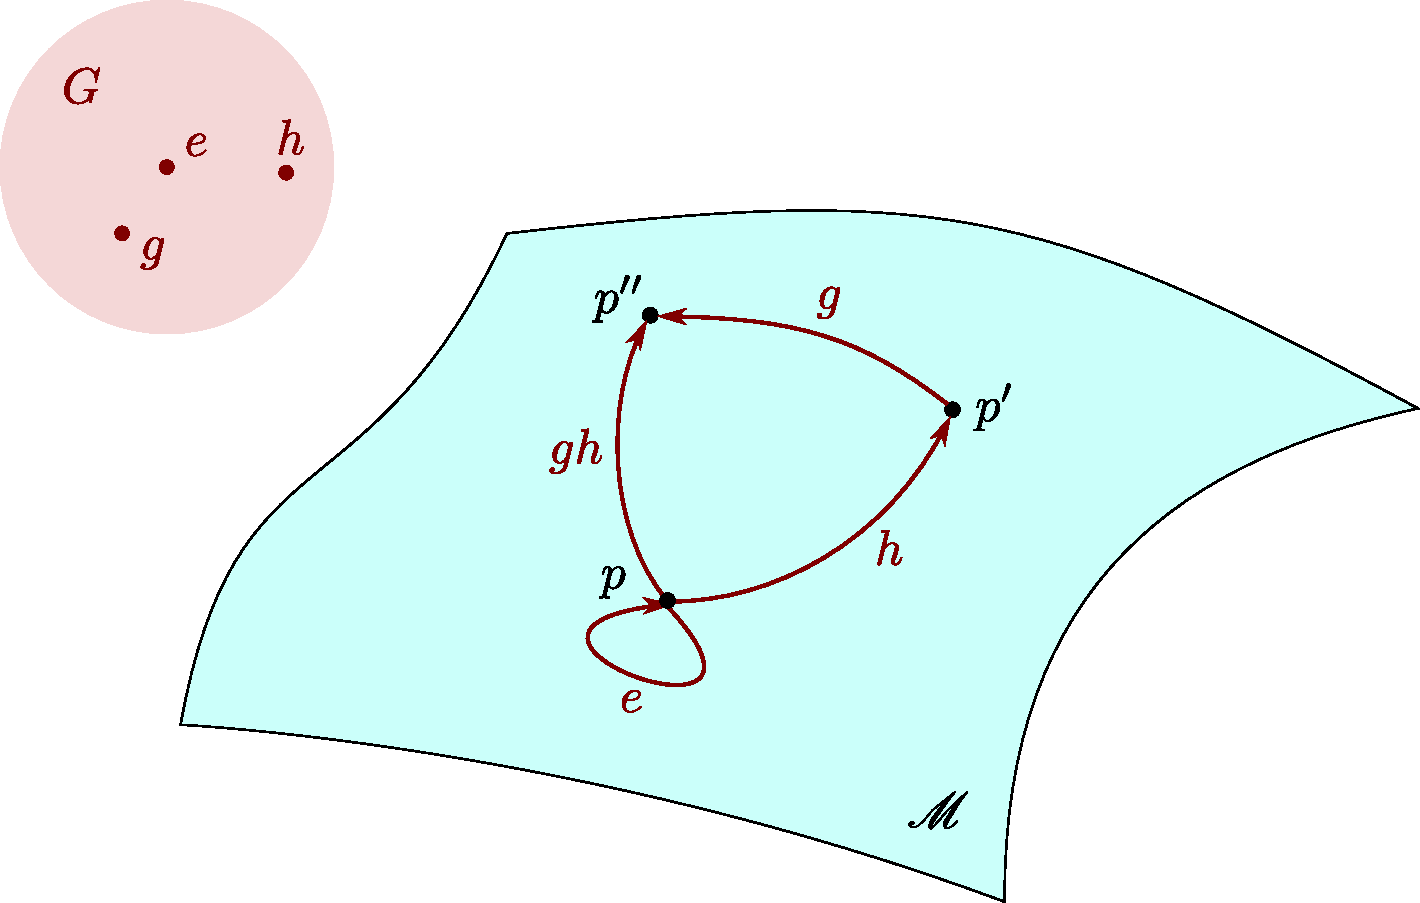
\includegraphics[width=0.8\textwidth]{def_group_action.pdf}}
\caption[]{\label{f:neh:group_action} \footnotesize
Group action of $G$ on $\M$.}
\end{figure}


\subsection{Spacetime symmetries} \label{s:neh:symmetries}

Symmetries of spacetime are described in a coordinate-independent way by means of
a (symmetry) group acting on the spacetime manifold $\M$.
Through this action, each transformation belonging to the group displaces points within $\M$ and one demands that the metric $\w{g}$ is invariant under such displacement.
More precisely, given
a group $G$, a \defin{group action}\index{group!action} of $G$ on $\M$ is a map\footnote{Do no confuse the generic element $g$ of the group $G$ with the metric tensor $\w{g}$.}
\be
	\begin{array}{rccl}
	\Phi: & G\times \M & \longrightarrow & \M \\
		& (g,p) & \longmapsto & \Phi(g,p) =: \Phi_g(p)
	\end{array}
\ee
such that (cf. Fig.~\ref{f:neh:group_action})
\begin{itemize}
\item if $e$ is the identity element of $G$, then
$\forall p\in \M,\  \Phi_e(p) = p$ ;
\item $\forall (g,h) \in G^2,\  \forall p\in\M,\  \Phi_g(\Phi_h(p)) = \Phi_{gh}(p)$, where $gh$ stands for the product of $g$ by $h$ according to the group law of
$G$.
\end{itemize}
The \defin{orbit}\index{orbit!under a group action} of a point $p\in\M$ is the set $\{g(p),\ g\in G\}\subset\M$, i.e. the set of points which are connected to $p$ by some group transformation. One says that $p$ is a
\defin{fixed point}\index{fixed!point} of the group action if its orbit is
reduced to $\{p\}$.

An important class of group actions are those for which $G$ is a 1-dimensional
\emph{Lie group}, i.e. a ``continuous'' group (actually a ``differentiable'' group).
Then around $e$, the elements of $G$ can be labelled by a parameter $t\in \R$, such that $g_{t=0} = e$. It is then
common to use the shorthand notation
\be
        \Phi_t := \Phi_{g_t} .
\ee
Because $G$ is a 1-dimensional Lie group, the orbit of a given point $p\in\M$ under the group action is then either $\{p\}$ (when $p$ is fixed point of the
group action) or a curve of $\M$. In the latter case,
$t$ is a natural parameter along the curve (cf. Fig.~\ref{f:neh:orbit_group}). The tangent vector corresponding to that parameter is called the \defin{generator of the group} $G$
(associated with the $t$-parametrization). At each point $p$ of
an orbit, it is given by
\be \label{e:neh:xi_dxdt}
    \w{\xi} = \frac{\D\w{x}}{\D t} ,
\ee
where $\D\w{x}$ is the infinitesimal vector connecting the point $p$ to the point
$\Phi_{\D t}(p)$ (cf. Sec.~\ref{s:bas:vectors} and Fig.~\ref{f:neh:orbit_group}).
We have then
\begin{greybox}
The action of $G$ on $\M$ limited to infinitesimal transformations of parameter
$\D t$ around the identity ($\D t =0$) amounts to translations along the infinitesimal vector $\D t\, \w{\xi}$.
\end{greybox}

\begin{figure}
\centerline{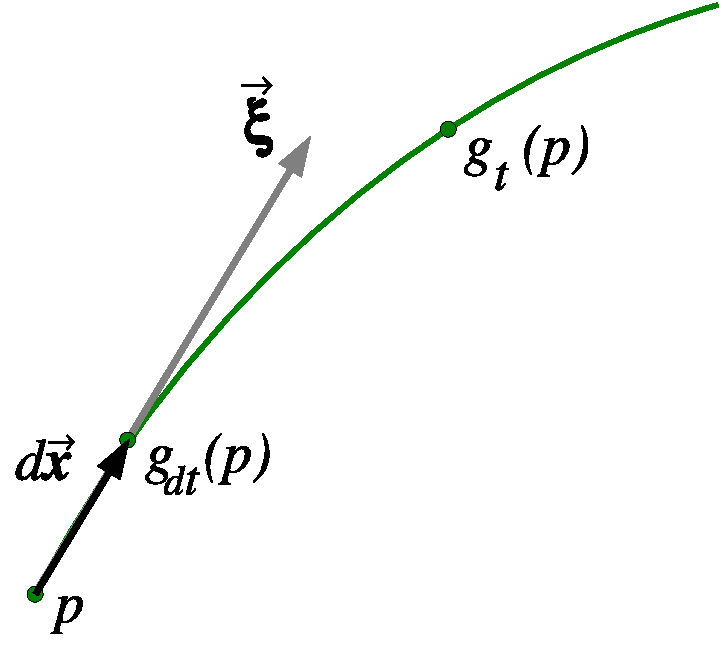
\includegraphics[height=0.25\textheight]{def_orbit_group.pdf}}
\caption[]{\label{f:neh:orbit_group} \footnotesize
Orbit of a point $p$ under the action $\Phi$ of a 1-dimensional Lie group, parametrized
by $t\in\R$. The vector $\w{\xi} = \D\w{x}/\D t$ is the group
generator associated with this parameter.}
\end{figure}

A 1-dimensional Lie group $G$ is said to be a
\defin{symmetry group}\index{symmetry!group}\index{group!symmetry --}
of the spacetime $(\M,\w{g})$ if there is an action $\Phi$ of $G$ on $\M$
such that for any value of the parameter $t$ of $G$,
$\Phi_t$ is an \defin{isometry}\index{isometry} of $(\M,\w{g})$, i.e. $\Phi_t$
preserves the ``distances'' and more generally the ``scalar products'' on
$(\M,\w{g})$, in the following sense: for any $p\in\M$ and any pair of points $(q,r)$
infinitely close to $p$, we shall have
\be \label{e:neh:isometry_dx}
    \left.\w{g}\right| _{\Phi_t(p)}(\D\w{x}', \D\w{y}') =
        \left.\w{g}\right| _{p}(\D\w{x}, \D\w{y}) ,
\ee
with the infinitesimal displacement vectors $\D\w{x} := \vp{pq}$, $\D\w{y} := \vp{pr}$,
$\D\w{x}' := \vp{\Phi_t(p)\Phi_t(q)}$ and $\D\w{y}' := \vp{\Phi_t(p)\Phi_t(r)}$
(cf. Sect.~\ref{s:fra:spacetime}).
Now, by definition, $\D\w{x}'$ is nothing but the pushforward
of the vector $\D\w{x}\in T_p\M$ to the tangent space
$T_{\Phi_t(p)}\M$ by the map $\Phi_t$
(cf. Sec.~\ref{s:bas:Lie_der_vector} in Appendix~\ref{s:bas}),
and similarly $\D\w{y}'$ is the pushforward of $\D\w{y}$ by $\Phi_t$:
\[
    \D\w{x}' = \Phi_t^*(\D\w{x}) \quad\mbox{and}\quad
    \D\w{y}' = \Phi_t^*(\D\w{y}) .
\]
By rescaling by infinitely small parameters (using the bilinearity of $\w{g}$),
it is clear that (\ref{e:neh:isometry_dx})
holds for finite vectors as well, so that we may say that $\Phi_t$ is an
isometry of $(\M,\w{g})$ iff
\be \label{e:neh:isometry}
    \forall p\in\M,\  \forall (\w{u},\w{v}) \in (T_p\M)^2,\quad
    \left. \w{g}\right| _{\Phi_t(p)} \left(\Phi_t^*(\w{u}), \Phi_t^*(\w{v})\right) =
    \left. \w{g}\right| _{p} (\w{u},\w{v}) ,
\ee
where $\Phi_t^*(\w{u})$ (resp. $\Phi_t^*(\w{v})$) is the pushforward of the vector $\w{u}\in T_p\M$ (resp. $\w{v}\in T_p\M$)
to the tangent space $T_{\Phi_t(p)}\M$ by $\Phi_t$ [cf. Eq.~(\ref{e:bas:def_Phi_eps})].
Given the definition (\ref{e:bas:def_pullback}) of the pullback of
a bilinear form, we may reexpress the isometry condition (\ref{e:neh:isometry})
in terms of the
pullback of $\w{g}$ by $\Phi_t$:
\be \label{e:neh:isometry_pullback}
    \Phi_t^*\w{g} = \w{g} .
\ee
Now, according the definition (\ref{e:bas:def_Lie_der_covar}) of the Lie
derivative, we have
\be
    \Lie{\xi} \w{g} := \lim_{t \rightarrow 0} \frac{1}{t}
    \left( \Phi_\varepsilon^*\w{g} - \w{g} \right) .
\ee
If $G$ is a symmetry group of $(\M,\w{g})$ with generator $\w{\xi}$,
(\ref{e:neh:isometry_pullback}) leads then to
$\Lie{\xi}\w{g} = 0$. The reverse is true by integration. Hence
we conclude:
\begin{greybox}
A 1-dimensional Lie group $G$
is a symmetry group of the spacetime $(\M,\w{g})$ iff the Lie derivative
of the metric tensor along the generator $\w{\xi}$ of $G$
vanishes identically:
\be \label{e:neh:Lie_xi_g}
    \encadre{\Lie{\xi}\w{g} = 0 } .
\ee
The vector field $\w{\xi}$ is then called a \defin{Killing vector}\index{Killing!vector field}
of $(\M,\w{g})$.
\end{greybox}
Expressing the Lie derivative via Eq.~(\ref{e:bas:Lie_der_comp_nab}) of Appendix~\ref{s:bas},
we see immediately that Eq.~(\ref{e:neh:Lie_xi_g}) is equivalent to the so-called
\defin{Killing equation}\index{Killing!equation}:
\be \label{e:neh:Killing_equation}
    \encadre{ \nabla_\alpha \xi_\beta + \nabla_\beta \xi_\alpha = 0 }.
\ee

\subsection{Definition and examples of Killing horizons} \label{s:neh:def_Killing_hor}

\begin{greybox}
A \defin{Killing horizon}\index{Killing!horizon}\index{horizon!Killing --} is
a null hypersurface $\Hor$ such that a Killing vector field $\w{\xi}$ of $(\M,\w{g})$
is normal to it.
\end{greybox}

Thus the existence of a Killing horizon requires that the spacetime $(\M,\w{g})$ has
some continuous symmetry
(usually stationarity), namely that it is invariant under the action of a
1-parameter group, as described in Sec.~\ref{s:neh:symmetries}.
A definition equivalent to the above one is then:
\begin{greybox}
A \defin{Killing horizon} is a null
hypersurface $\Hor$ whose null geodesic generators are orbits of a
1-parameter group of isometries of $(\M,\w{g})$.
\end{greybox}

\begin{remark}
The above definition implies that the Killing vector field $\w{\xi}$ is null
and non-vanishing on $\Hor$:
\be \label{s:neh:xi_on_KH}
    \left. \w{\xi}\cdot\w{\xi} \right| _{\Hor} = 0 \qquad\mbox{and}\qquad
    \left. \w{\xi} \right| _{\Hor} \not= 0 .
\ee
Indeed, if $\w{\xi}$ is vanishing at some point of $\Hor$, it cannot be
considered as a normal vector to $\Hor$.
\end{remark}

We shall see in Chap.~\ref{s:sta} that in a stationary spacetime, a black hole
event horizon must be a Killing horizon.

\begin{figure}
\centerline{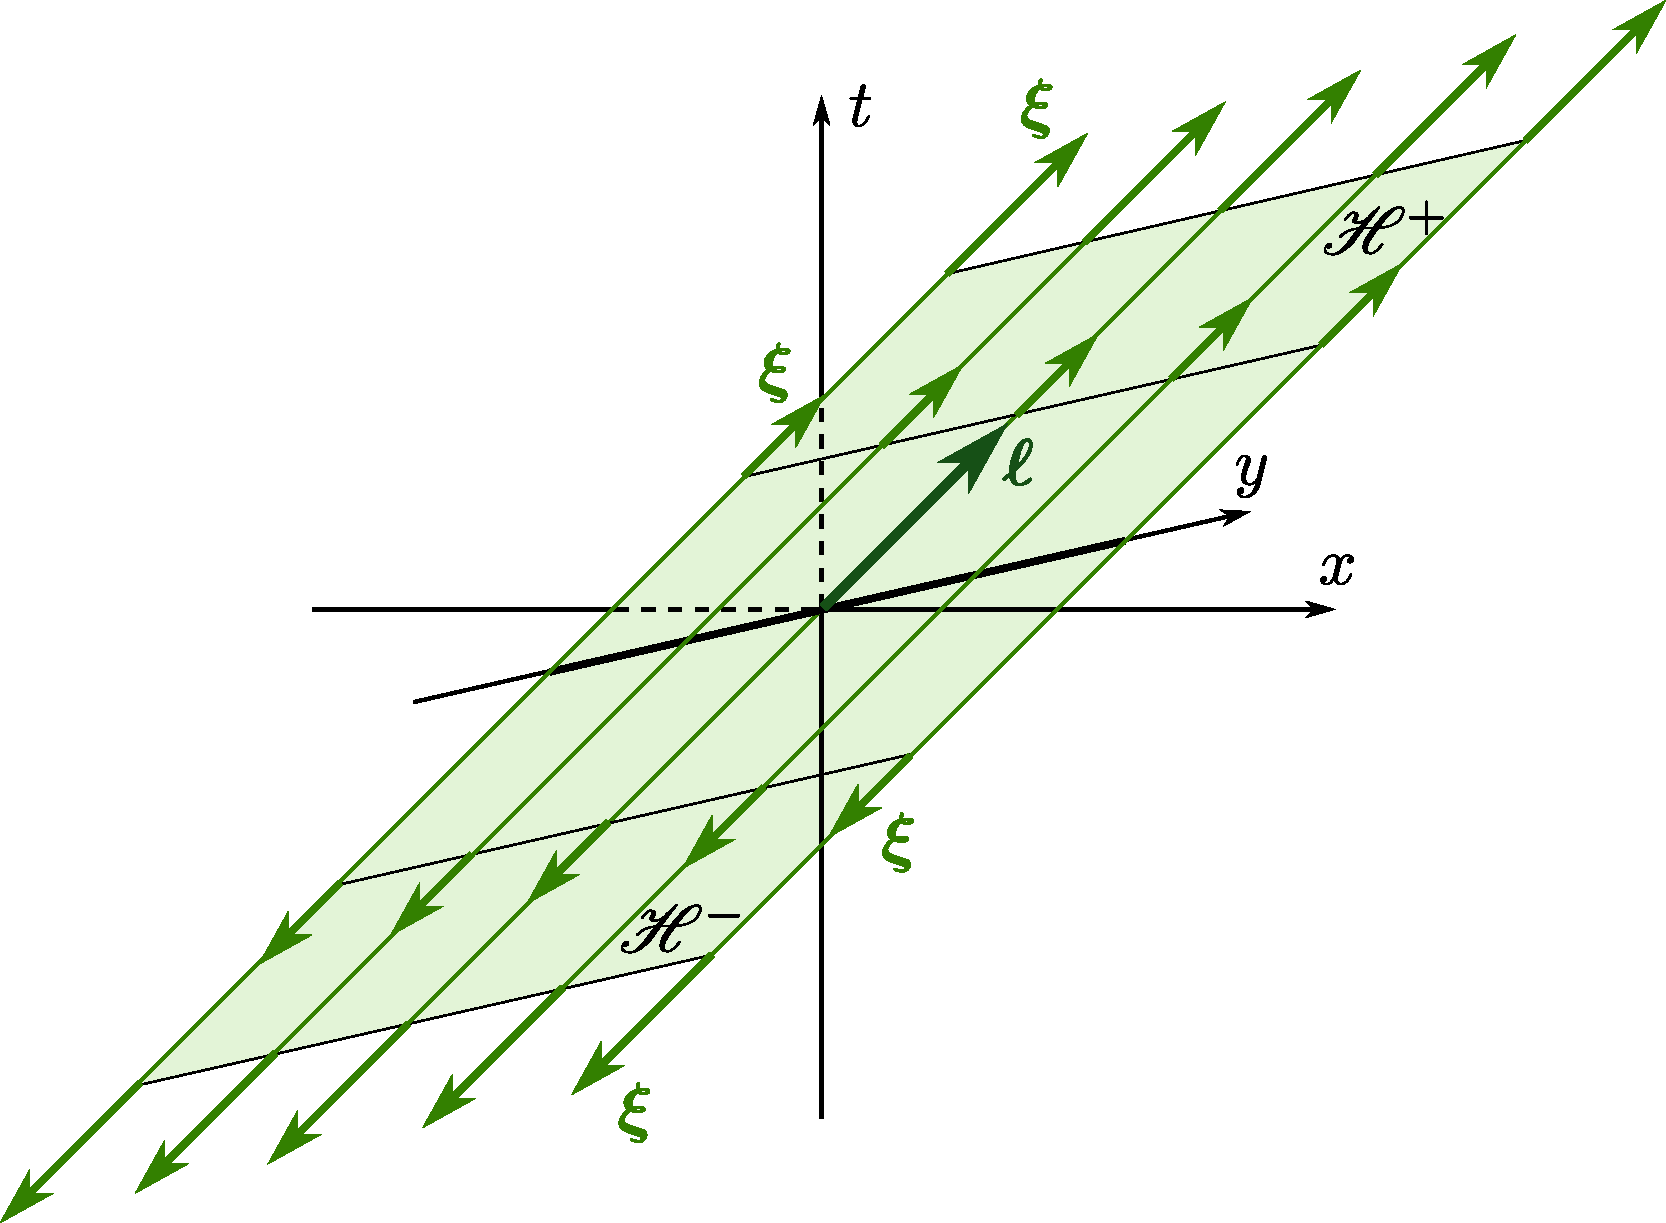
\includegraphics[width=0.6\textwidth]{def_hplaneKilling-boost.pdf}}
\caption[]{\label{f:neh:hplaneKilling-boost} \footnotesize
Null half-hyperplanes $\Hor^+$ and $\Hor^-$ as Killing horizons for the
Killing vector field $\w{\xi}=x \wpar_t + t \wpar_x$ generating Lorentz boosts
in Minkowski spacetime. The green lines are the null geodesic generators of
$\Hor$, while the thick black line (actually a 2-plane) marks the location
where $\w{\xi}=0$.}
\end{figure}

\begin{example}[null hyperplane as a translation-Killing horizon]
\label{x:neh:transKH}
Let us consider the null hyperplane of Minkowski spacetime $\Hor$ discussed in
Examples~\ref{x:def:null_hyp}, \ref{x:def:null_hyp2} and \ref{x:def:null_hyp3}
of Chap.~\ref{s:def}.
$\Hor$ is defined by the equation $t=x$. The vector field
\be
    \w{\xi} := \wpar_t + \wpar_x
\ee
is a Killing vector of Minkowski spacetime: $\w{\xi}$ is the generator of
translations in the direction $\wpar_t + \wpar_x$, and these translations constitute a
1-dimensional subgroup of the Poincaré group --- the symmetry group of Minkowski
spacetime. We note that $\w{\xi}$ coincides with the null vector $\wl$
defined by Eq.~(\ref{e:def:wl_null_hyperplane}). Since $\wl$ is
normal to $\Hor$, we conclude immediately that $\Hor$ is a Killing horizon
with respect to $\w{\xi}$.
\end{example}

\begin{example}[null hyperplane as a boost-Killing horizon]
\label{x:neh:boostKH}
Let us consider again the null hyperplane $\Hor$, but setting
\be
    \w{\xi} := x \wpar_t + t \wpar_x ,
\ee
which defines another Killing vector of Minkowski spacetime: $\w{\xi}$ is indeed the
generator of the 1-parameter group of Lorentz boosts\index{boost} in the $(t,x)$ plane.
On $\Hor$ we have (cf. Fig.~\ref{f:neh:hplaneKilling-boost}):
\[
    \w{\xi} \equalH t (\wpar_t + \wpar_x) \equalH t \, \wl ,
\]
where $\wl$ is the null normal to $\Hor$ defined by
Eq.~(\ref{e:def:wl_null_hyperplane}) and the notation $\equalH$ means that the equality holds only on $\Hor$. We conclude that $\w{\xi}$ is a normal to
the null hypersurface $\Hor$ as soon as $t\not=0$. Therefore, we may split
$\Hor\setminus\{t=0\}$ in two open half-hyperplanes (cf. Fig.~\ref{f:neh:hplaneKilling-boost}):
\[
    \Hor^+ := \{ p\in\Hor,\quad t(p) > 0 \} \quad\mbox{and}\quad
    \Hor^- := \{ p\in\Hor,\quad t(p) < 0 \}
\]
and each null hypersurface $\Hor^+$ and $\Hor^-$ is a Killing horizon with
respect to $\w{\xi}$.
\end{example}

\begin{example}[null hyperplane as a null-rotation-Killing horizon]
\label{x:neh:nullrotKH}
Another example of Killing horizon is still provided by the null hyperplane
$\Hor$ considered above, but this time with the Killing vector
\be \label{e:neh:xi_null_rotation}
   \w{\xi} := y( \wpar_t + \wpar_x ) + (t-x)\wpar_y .
\ee
This vector is indeed the generator of
null rotations leaving the plane
$\mathrm{Span}(\wl,\wpar_z)$ strictly invariant (cf. e.g. Sec.~6.4.5 of
Ref.~\cite{Gourg13}), $\wl$ being the null normal of $\Hor$ defined by
Eq.~(\ref{e:def:wl_null_hyperplane}), and these null rotations form a
1-dimensional subgroup of the Lorentz group, and thereby
a symmetry group of Minkowski spacetime. It is also immediate to check that
the vector $\w{\xi}$ defined by (\ref{e:neh:xi_null_rotation}) obeys
Killing equation [Eq.~(\ref{e:neh:Killing_equation})].
On $\Hor$, $t-x=0$, so that
(\ref{e:neh:xi_null_rotation}) reduces to
\[
    \w{\xi}  \equalH y ( \wpar_t + \wpar_x )  \equalH y \, \wl .
\]
It follows that $\w{\xi}$ is a null normal to $\Hor$ as soon as $y\not=0$.
We may then split $\Hor\setminus\{y=0\}$ in two open half-hyperplanes (cf. Fig.~\ref{f:neh:hplaneKilling-nullrot}):
\[
    \Hor_1 := \{ p\in\Hor,\quad y(p) < 0 \} \quad\mbox{and}\quad
    \Hor_2 := \{ p\in\Hor,\quad y(p) > 0 \} ,
\]
each of them being a Killing horizon with
respect to $\w{\xi}$.
\end{example}

\begin{figure}
\centerline{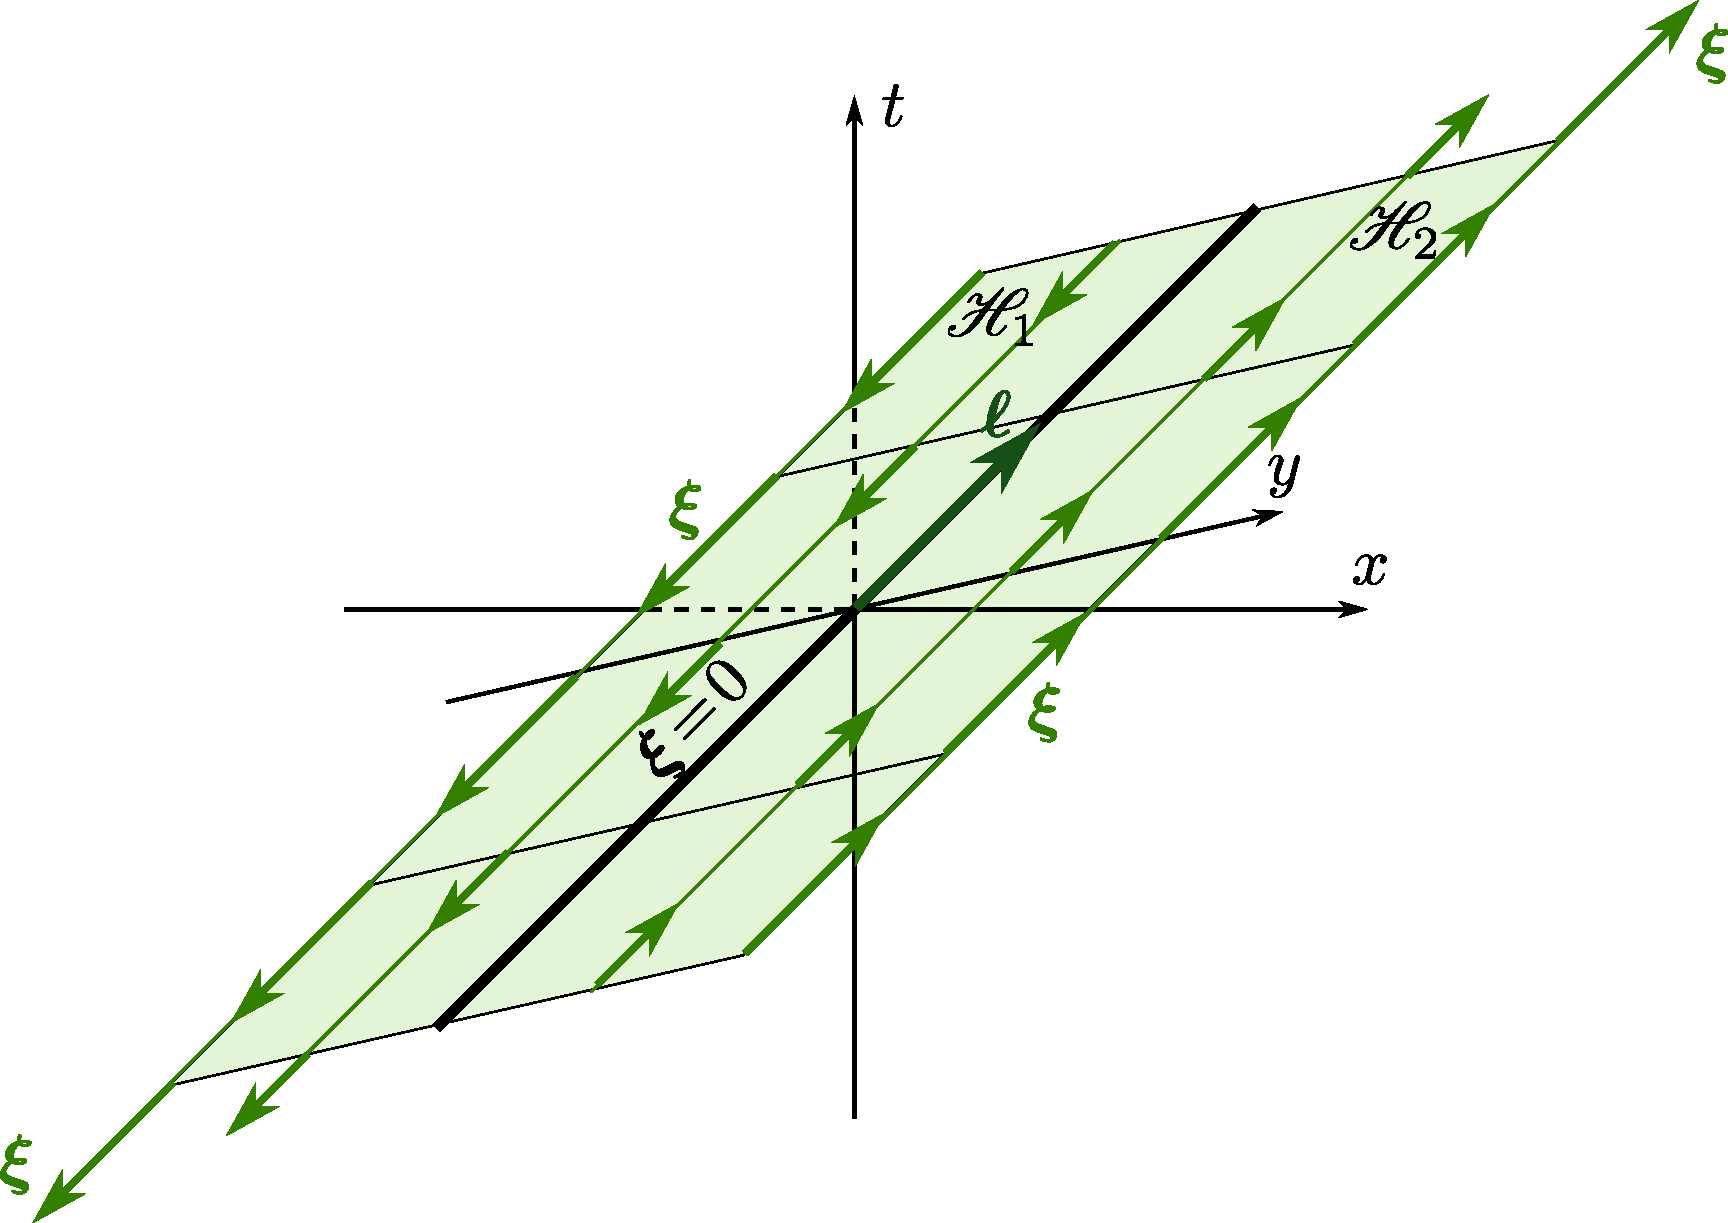
\includegraphics[width=0.6\textwidth]{def_hplaneKilling-nullrot.pdf}}
\caption[]{\label{f:neh:hplaneKilling-nullrot} \footnotesize
Null half-hyperplanes $\Hor_1$ and $\Hor_2$ as Killing horizons for the
Killing vector field $\w{\xi}=y( \wpar_t + \wpar_x ) + (t-x)\wpar_y$
generating null rotations
in Minkowski spacetime. The green lines are the null geodesic generators of
$\Hor$, while the thick black line (actually a 2-plane) marks the location
where $\w{\xi}=0$.}
\end{figure}

\begin{example}[light cone as a counter-example]
The future light cone introduced in Example~\ref{x:def:light_cone} of Chap.~\ref{s:def} is \emph{not} a
Killing horizon of Minkowski spacetime: it is invariant under the action
of the Lorentz group, but its null generators are not invariant
under the action of a single 1-dimensional subgroup of the Lorentz group.
Actually the future light cone is an example of a more general structure,
which Brandon Carter \cite{Carte67,Carte69} has termed a
\defin{local isometry horizon}\index{local!isometry horizon}\index{isometry!horizon}\index{horizon!local isometry --}: a null hypersurface that is invariant under
some group $G$ of isometries (here: the Lorentz group) and such that each null
geodesic generator is an orbit under some 1-dimensional subgroup of $G$ (here: using Minkowskian spherical
coordinates $(t,r,\th,\ph)$,
the null geodesic generator through the point of coordinates $(1,1,\th_0,\ph_0)$
is the orbit of this point under the subgroup of boosts in the plane
$(\th,\ph) = (\th_0,\ph_0)$). A Killing horizon is a local isometry horizon
for which $\dim G = 1$.
\end{example}


\begin{example}[Schwarzschild horizon]
Given the expression (\ref{e:def:wl_Schw_hor}) for the null normal $\wl$
of the family of hypersurfaces $\Hor_u$ and the fact that the Schwarzschild
horizon $\Hor$ is defined by $r=2m$, we have
\be \label{e:neh:wl_wpt_Schw_hor}
    \wl \equalH \wpar_t .
\ee
Now the vector field $\wpar_t$ is clearly a Killing vector of metric $\w{g}$
as given by (\ref{e:def:Schw_metric}), since none of the metric components
$g_{\alpha\beta}$ depends upon $t$. Hence (\ref{e:neh:wl_wpt_Schw_hor})
shows that the Schwarzschild horizon is a Killing horizon. By the way,
Eq.~(\ref{e:neh:wl_wpt_Schw_hor}) was our motivation for the choice of the
null normal $\wl$ performed in Example~\ref{x:def:Schw_hor2} of Chap.~\ref{s:def}.
\end{example}

\begin{hist}
The concept of Killing horizon has been introduced by Brandon Carter in
1966 \cite{Carte66,Carte67} and developed in an article published in
1969 \cite{Carte69}. The properties of Killing horizons have been
studied in detail by Robert H. Boyer, in an article prepared posthumously from his notes
by J.~Ehlers and J.L.~Stachel and published in 1969 \cite{Boyer69},
leading to the concept of \emph{bifurcate Killing horizon}, to be discussed in
Sec.~\ref{s:sta:bifur_Killing_hor}.
\end{hist}

\subsection{Killing horizons as non-expanding horizons}

Let $\Hor$ be a Killing horizon with cross-sections that are closed manifolds,
i.e. the topology of $\Hor$ is (\ref{e:def:H_topology}). Let us select the null normal $\wl$
that coincides with the Killing vector $\w{\xi}$ on $\Hor$:
$\wl \equalH \w{\xi}$.
Equation~(\ref{e:neh:Lie_xi_g}) then implies:
\[
    \Lie{\el} \w{g} \equalH 0 .
\]
Let $\Sp$ be a cross-section of $\Hor$; since $\w{q}$ is the metric induced by $\w{g}$
on $\Sp$, we deduce immediately that
\[
    \Lie{\el} \w{q} = 0 .
\]
From the definition (\ref{e:def:Theta}), it follows that the expansion rate
tensor of $\Sp$ vanishes identically:
\be \label{e:neh:Theta_zero_KillingH}
    \w{\Theta} = 0 .
\ee
In particular we have
\[
    \theta_{(\wl)} = 0 .
\]
We conclude that
\begin{greybox}
Any Killing horizon with closed-manifold cross-sections is a non-expanding horizon.
\end{greybox}
Moreover, (\ref{e:neh:Theta_zero_KillingH}) shows that $\w{\Theta}$ vanishes
for all Killing horizons, while to get the same result on a generic non-expanding
horizon, one has to assume that the null energy condition holds on $\Hor$.

\subsection{The zeroth law of black hole mechanics}

Let us show that, on a Killing horizon, modulo some mild energy condition,
the non-affinity coefficient $\kappa$
(cf. Sec.~\ref{s:def:geod_gener})
of the null normal $\wl$ coinciding with a Killing vector is constant.

First of all, since $\wl$ is a symmetry generator on $\Hor$, we have
\be
    \Lie{\el} \kappa = 0 ,
\ee
which means that $\kappa$ is constant along the field lines of $\wl$ (i.e. the
null geodesic generators of $\Hor$). It could however vary from a field line to another
one. To show that this is not the case, let us consider a cross-section
$\Sp$ of $\Hor$ and project the contracted Ricci identity (\ref{e:def:contract_Ricci_ident})
onto it:
\[
    \nabla_\mu \Theta^\mu_{\ \, \nu} q^\nu_{\ \, \alpha} + \el^\mu \nabla_\mu \omega_\nu q^\nu_{\ \, \alpha}
       - \nabla_\nu \left( \theta_{(\wl)} + \kappa \right) q^\nu_{\ \, \alpha}
        + \left( \theta_{(\wl)} + \kappa \right) \omega_\nu q^\nu_{\ \, \alpha}
        - \Theta_{\alpha\mu} k^\nu \nabla_\nu \el^\mu \nonumber \\
     = R_{\mu\nu} \el^\mu q^\nu_{\ \, \alpha}, \nonumber
\]
where we have used $\Theta_{\nu\mu}  q^\nu_{\ \, \alpha} = \Theta_{\alpha\mu}$
and $\el_\nu q^\nu_{\ \, \alpha} = 0$.
Now, since $\Hor$ is a non-expanding horizon, we may set $\w{\Theta}=0$ and
$\theta_{(\wl)} =0$, so that the above equation reduces to
\be \label{e:neh:zeroth_law_step1}
    \el^\mu \nabla_\mu \omega_\nu q^\nu_{\ \, \alpha} - \nabla_\nu \kappa \, q^\nu_{\ \, \alpha}
    + \kappa  \, \omega_\nu q^\nu_{\ \, \alpha} = R_{\mu\nu} \el^\mu q^\nu_{\ \, \alpha} .
\ee
Let us express $\el^\mu \nabla_\mu \omega_\nu$ in terms of the Lie derivative
of $\w{\omega}$ along $\wl$ via formula (\ref{e:bas:Lie_der_comp_nab}) of Appendix~\ref{s:bas}:
\[
    \Liec{\el}\omega_\nu = \el^\mu \nabla_\mu \omega_\nu + \omega_\mu \nabla_\nu \el^\mu .
\]
Now, since $\wl$ is a symmetry generator on $\Hor$, we have
\be
    \Lie{\el}\w{\omega} \equalH 0 ,
\ee
so that
\[
    \el^\mu \nabla_\mu \omega_\nu \equalH - \omega_\mu \nabla_\nu \el^\mu .
\]
Accordingly, Eq.~(\ref{e:neh:zeroth_law_step1}) becomes successively
\bea
   & & - \omega_\mu \nabla_\nu \el^\mu  q^\nu_{\ \, \alpha}
     - \nabla_\nu \kappa \, q^\nu_{\ \, \alpha}
    + \kappa  \, \omega_\nu q^\nu_{\ \, \alpha} = R_{\mu\nu} \el^\mu q^\nu_{\ \, \alpha} \nonumber \\
   & &  - \omega_\mu \left(\Theta_\nu^{\ \, \mu}
        + \omega_\nu \el^\mu - \el_\nu k^\sigma \nabla_\sigma \el^\mu \right) q^\nu_{\ \, \alpha}
     - \nabla_\nu \kappa \, q^\nu_{\ \, \alpha}
    + \kappa  \, \omega_\nu q^\nu_{\ \, \alpha} = R_{\mu\nu} \el^\mu q^\nu_{\ \, \alpha} \nonumber \\
   & &   - \omega_\mu
   \underbrace{\Theta_\alpha^{\ \, \mu}}_{0}
        - \underbrace{\omega_\mu \el^\mu}_{\kappa} \omega_\nu q^\nu_{\ \, \alpha}
     - \nabla_\nu \kappa \, q^\nu_{\ \, \alpha}
    + \kappa  \, \omega_\nu q^\nu_{\ \, \alpha} = R_{\mu\nu} \el^\mu q^\nu_{\ \, \alpha}  \nonumber \\
   & &
   - \nabla_\nu \kappa \, q^\nu_{\ \, \alpha} = R_{\mu\nu} \el^\mu q^\nu_{\ \, \alpha} , \nonumber
\eea
where we have used (\ref{e:def:nab_l_Theta}) to get the second line,
the identity
$\el_\nu q^\nu_{\ \, \alpha} = 0$ to get the third one and
(\ref{e:def:omega_l_kappa}) to substitute $\kappa$ for
$\omega_\mu \el^\mu$.
In the above equation appears the covariant derivative of $\kappa$ along $\Sp$,
which we denote by $\DS$:
\be
    \DSc_\alpha \kappa := \nabla_\nu \kappa \, q^\nu_{\ \, \alpha} .
\ee
Using the Einstein equation (\ref{e:bas:Einstein_eq_n}), we may then rewrite
the above relation as
\[
    \DSc_\alpha \kappa = -  \frac{2}{n-2}\,\Lambda\,
    \underbrace{g_{\mu\nu}  \el^\mu q^\nu_{\ \, \alpha}}_{\el^\mu q_{\mu\alpha} = 0}
    - 8\pi \Big( T_{\mu\nu} \el^\mu q^\nu_{\ \, \alpha}
    - \frac{1}{n-2}\,  T \, \underbrace{g_{\mu\nu}  \el^\mu q^\nu_{\ \, \alpha}}_{\el^\mu q_{\mu\alpha} = 0} \Big) ,
\]
i.e.
\be \label{e:neh:DS_kappa_W}
    \DSc_\alpha \kappa = - 8\pi T_{\mu\nu} \el^\mu q^\nu_{\ \, \alpha} .
\ee
To go further, we shall assume that matter and the non-gravitational fields
obey the
\defin{null dominant energy condition}\index{null!dominant energy condition}\index{energy!condition!null dominant--}:
\be
   \begin{array}{ll}
    \w{W} := - \vw{T}(\wl, .) \ & \mbox{is future-directed null or timelike} \\
    & \mbox{for any future-directed null vector $\wl$} .
    \end{array}
\ee
In the above equation, $\vw{T}(\wl, .)$ stands for the vector field
that is the metric dual of the 1-form $\w{T}(\wl, .)$; in index notation,
\[
    W^\alpha = - g^{\alpha\nu} T_{\mu\nu}\el^\mu = - T_\mu^{\ \, \alpha} \el^\mu .
\]
Note that the null dominant energy condition implies the null energy condition
discussed in Sec.~\ref{s:neh:NEH_Theta_zero}, since
\[
    \w{T}(\wl, \wl) = - \w{W}\cdot\wl \geq 0 ,
\]
the inequality holding because both $\w{W}$ and $\wl$ are future-directed.

The null dominant energy condition is implied by continuity by the
\defin{dominant energy condition}\index{dominant energy condition}\index{energy!condition!dominant--}:
\be
   \begin{array}{ll}
    \w{W} := - \vw{T}(\w{u}, .) \ & \mbox{is future-directed null or timelike} \\
    & \mbox{for any future-directed timelike vector $\w{u}$} .
    \end{array}
\ee
Physically, the dominant energy condition states that, with respect to any
observer (represented by its 4-velocity $\w{u}$, which is future-directed timelike),
the energy of matter and non-gravitational fields, moves at a speed
at most equal to $c$.

We note that in the right-hand side of (\ref{e:neh:DS_kappa_W}), there appears the
orthogonal projection of $\w{W}$ onto $\Sp$ (more precisely its metric dual).
If we assume the null dominant energy condition, the null energy condition
holds and we have, according to (\ref{e:neh:T_l_l_zero}),
\[
    \wl \cdot \w{W} = - \w{T}(\wl, \wl) = 0 ,
\]
This implies that the vector $\w{W}$ is tangent to $\Hor$. The latter
being a null hypersurface, $\w{W}$ must then be
either collinear to $\wl$ or spacelike (cf. the lemma in Sec.~\ref{s:def:spacelike_sections}).
Now, according to the null dominant energy condition, $\w{W}$ cannot be
spacelike. We conclude that $\w{W}$ is collinear to $\wl$. Consequently its
orthogonal projection onto $\Sp$ is zero:
\[
    q^\alpha_{\ \, \nu} W^\nu = - q^\alpha_{\ \, \nu} T_\mu^{\ \, \nu} \el^\mu = 0 .
\]
Hence the right-hand side of (\ref{e:neh:DS_kappa_W}) vanishes identically
and we are left with
\[
    \DSc_\alpha \kappa = 0 .
\]
This means that $\kappa$ is constant over $\Sp$. Given that $\kappa$ is
constant along each null geodesic generator of $\Hor$, this completes the demonstration
that $\kappa$ is constant over $\Hor$. More precisely, we have shown that
\begin{greybox}
If matter and the non-gravitational fields obey the dominant energy condition
on the Killing horizon $\Hor$, then the non-affinity coefficient $\kappa$
associated with the null normal coinciding with the Killing vector field on
$\Hor$ is constant over $\Hor$:
\be \label{e:neh:zeroth_law}
    \encadre{\kappa = \mathrm{const}.}
\ee
\end{greybox}
In the context of Killing horizons, the non-affinity coefficient $\kappa$ is
often called the horizon's \defin{surface gravity}\index{surface!gravity} and the result
(\ref{e:neh:zeroth_law}) is known as the
\defin{zeroth law of black hole mechanics}\index{zeroth law}. More precisely,
the latter states that the surface gravity of a black hole in equilibrium is
constant and we shall see in Chap.~\ref{s:sta} that the event horizon of a black hole in
equilibrium is a Killing horizon.

\begin{example}[null hyperplane as a translation-Killing horizon]
For the null hyperplane $\Hor$ considered in Example~\ref{x:neh:transKH} as a Killing horizon with respect to the translation group along its normal, we have
$\kappa = 0$, as already noticed in Example~\ref{x:def:null_hyp3} of Chap.~\ref{s:def}
[Eq.~(\ref{e:def:kappa_0_nullhyp})], which is obviously constant over $\Hor$.
\end{example}

\begin{example}[null hyperplane as a boost-Killing horizon]
Let us consider each of the null half-hyperplanes $\Hor^+$
and $\Hor^-$ of Example~\ref{x:neh:boostKH}, which are Killing horizons with
respect to the boost Killing vector $\w{\xi} = x \wpar_t + t \wpar_x$. On
$\Hor^+$, the future-directed null normal coinciding with this Killing vector
is $\wl^+ = t\,  \wl$, $\wl$ being the geodesic null normal defined by
$\wl:= \wpar_t + \wpar_x$ [cf. Eq.~(\ref{e:def:wl_null_hyperplane})].
Using $\kappa_{\wl} = 0$ and the scaling law (\ref{e:def:rescale_kappa}),
we get the non-affinity
coefficient associated with $\wl^+$ as $\kappa_+= \wnab_{\wl} t = \partial_t t + \partial_x t$, i.e.
\[
    \kappa_+ = 1 .
\]
On $\Hor^-$, $\w{\xi}$ is past-directed (cf. Fig.~\ref{f:neh:hplaneKilling-boost}).
Sticking to future-directed null normals, we shall then consider $\Hor^-$
as a Killing horizon with respect to the Killing vector field $-\w{\xi}$.
The future-directed null normal coinciding with $-\w{\xi}$ on $\Hor^-$ is then
$\wl^- = -t\,  \wl$, from which we deduce the non-affinity
coefficient associated with $\wl^-$:
\[
    \kappa_- = 1 .
\]
We check that $\kappa_+$ (resp.  $\kappa_-$) is constant over the Killing horizon $\Hor^+$ (resp. $\Hor^-$), in agreement with the result above.
\end{example}

\begin{example}[null hyperplane as a null-rotation-Killing horizon]
In Example~\ref{x:neh:nullrotKH}, we have introduced the Killing horizons
$\Hor_1$ and $\Hor_2$ with respect to the null-rotation Killing vector
$\w{\xi} = y( \wpar_t + \wpar_x ) + (t-x)\wpar_y$ of Minkowski spacetime.
On $\Hor_1$, $\w{\xi}$ is past-directed (cf. Fig.~\ref{f:neh:hplaneKilling-nullrot}),
so that we shall actually consider $\Hor_1$
as a Killing horizon with respect to the Killing vector field $-\w{\xi}$.
The future-directed null normal coinciding with $-\w{\xi}$ on $\Hor_1$ is then
$\wl_1 = - y\, \wl$. Since it is clearly constant along the null geodesic generators
of $\Hor_1$, we have $\wnab_{\wl_1}\wl_1 = 0$, hence the
associated non-affinity coefficient vanishes:
\[
    \kappa_1 = 0 .
\]
On $\Hor_2$, $\w{\xi}$ is future-directed (cf. Fig.~\ref{f:neh:hplaneKilling-nullrot})
and the null normal coinciding with it is $\wl_2 =  y\,  \wl$, whose non-affinity
coefficient is
\[
    \kappa_2 = 0 .
\]
\end{example}

\begin{example}[Schwarzschild and Kerr horizons]
We have found in Example~\ref{x:def:Schw_hor3} of Chap.~\ref{s:def} [cf. Eq.~(\ref{e:def:kappa_Schw_hor})]
that on a Schwarzschild horizon:
\[
  \kappa = \frac{1}{4m},
\]
which is clearly constant. But
this result is rather trivial since the Schwarzschild horizon is spherically
symmetric, so that no dependence of $\kappa$ on $\th$ nor $\ph$ could have been expected.
A much less trivial example is that of the event horizon of a Kerr black hole,
which we shall discuss in Chap.~\ref{s:ker}. This horizon is only axisymmetric,
so that a priori $\kappa$ could depend on $\th$. But it does not, as we shall
see in Sec.~\ref{s:ker:surf_grav}:
\[
    \kappa = \frac{\sqrt{m^2 - a^2}}{2m(m + \sqrt{m^2-a^2})} ,
\]
where $(m,a)$ are the two constant parameters of the Kerr solution. Note that for $a=0$,
we recover the Schwarzschild value: $\kappa= 1/(4m)$.
\end{example}

\begin{hist}
The constancy of $\kappa$ for a Killing horizon has been proven by S.W.~Hawking
in his lecture at the famous Les Houches School of Summer 1972 \cite{Hawki73} (p.~43).
It has also been proven without requiring the dominant energy condition, but
assuming axisymmetry by B.~Carter in his lecture at the same Les Houches School
\cite{Carte73b} (Theorem 8, p.~167).
A third proof of the constancy of $\kappa$ using the dominant energy condition
has also been given in 1973 by J.M.~Bardeen, B.~Carter and S.W.~Hawking
in their famous article \emph{The Four Laws of Black Hole Mechanics}
\cite{BardeCH73}.
\end{hist}

%%%%%%%%%%%%%%%%%%%%%%%%%%%%%%%%%%%%%%%%%%%%%%%%%%%%%%%%%%%%%%%%%%%%%%%%%%%%%%%%%%%%%%%%

\section{Summary}

Here is an inheritance diagram summarizing the main results of this chapter.
The vertical arrow means ``is a'', i.e. the element at the bottom of the arrow
is a special case of the element at the top of the arrow.
``NEC'' stands for ``Null Energy Condition''
and ``NDEC'' for ``Null Dominant Energy condition''.

\begin{center}

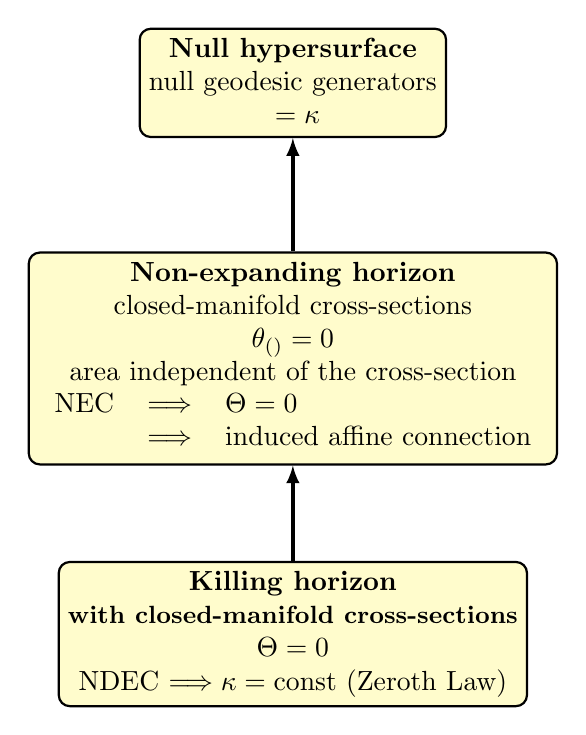
\begin{tikzpicture}
%\tikzstyle{boxst}=[rectangle,draw]
\tikzstyle{boxst}=[draw, thick, align=center, fill=yellow!20, rounded corners]
\tikzstyle{inherits}=[->,very thick,>=latex]
\node[boxst] (N) at (0,7) {\textbf{Null hypersurface}\\
null geodesic generators\\
$\wnab_{\wl}\wl = \kappa\wl$};
\node[boxst] (H) at (0,3.5) {\textbf{Non-expanding horizon}\\
closed-manifold cross-sections\\
$\theta_{(\wl)}=0$\\
area independent of the cross-section\\
\begin{tabular}{lcl}
NEC &$\Longrightarrow$ & $\w{\Theta}=0$ \\
 & $\Longrightarrow$ & induced affine connection
\end{tabular}
};
\node[boxst] (K) at (0,0) {\textbf{Killing horizon}\\
\textbf{\small with closed-manifold cross-sections}\\
$\w{\Theta}=0$ \\
NDEC $\Longrightarrow \kappa=\mathrm{const}$ (Zeroth Law)};
\draw[inherits] (H)--(N);
\draw[inherits] (K)--(H);
\end{tikzpicture}

\end{center}
